\subsection{Animieren eines Vehicles durch Interpolation}
\label{sub:animieren_eines_vehicles_durch_interpolation}
  Der zentrale Kerngedanke für die Animation der Vehicle-Bewegung ist die Interpolation von Distanzen zwischen zwei aufeinanderfolgenden Stationen A und B mit der Distanz  $d_{\triangle}$. Um zu verstehen, wie ein Vehicle zwischen den einzelnen Stationen interpoliert werden kann, soll Abbildung \ref{fig:interpolating_vehicle} helfen.

  \begin{figure}[htbp]
    \begin{center}
      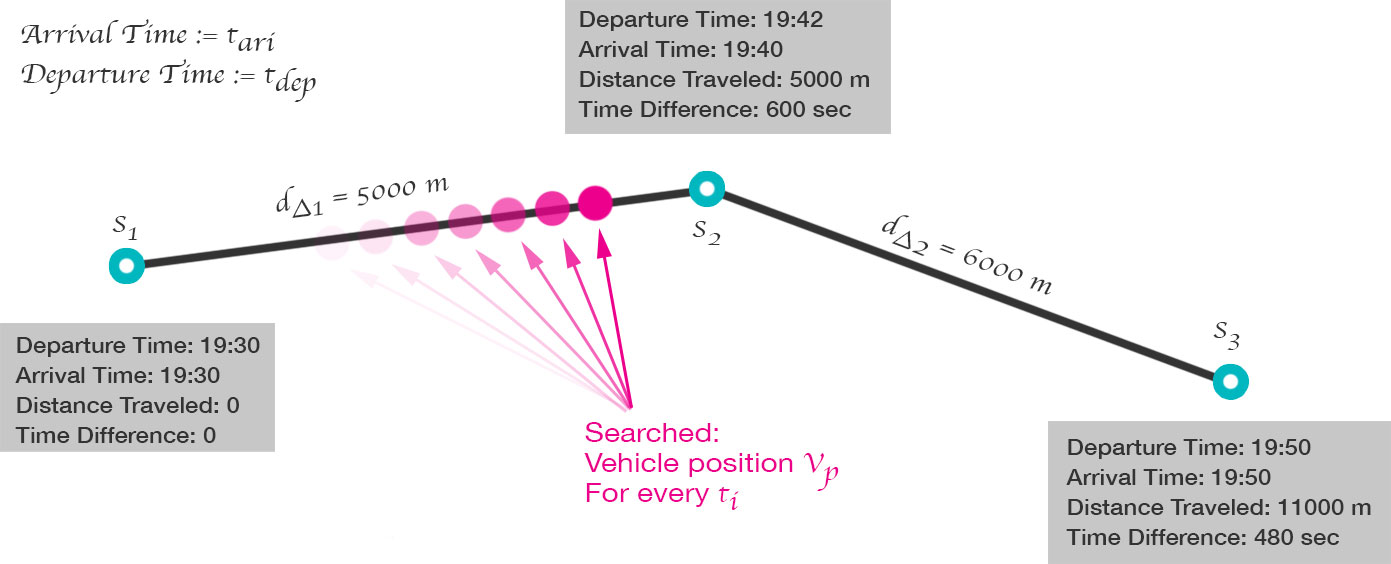
\includegraphics[width=0.9\textwidth]{interpolating_vehicle}
      \caption{Interpolation der Vehicle Position: $V_p$}
      \label{fig:interpolating_vehicle}
    \end{center}
  \end{figure}

  In den grauen Kästen der Grafik sind die Daten der einzelnen Stationen zu sehen. Diese kommen direkt aus der Datenbank oder werden vom Server vorberechnet und sind für die Berechnungen der Interpolation zwingend notwendig.
  \begin{itemize}[label={}]
    \item \textbf{Arrival Time:} Ankunftszeit $t_{ari}$ des Vehicles an der Station laut Fahrplan

    \item \textbf{Departure Time:} Abfahrtszeit $t_{dep}$ des Vehicles von der Station laut Fahrplan

    \item \textbf{Distance Traveled:} Bis zu dieser Station zurückzulegende Gesamtdistanz $d_S$

    \item \textbf{Difference Distance Traveled:} $d_\triangle$ ist die zurückzulegende Distanz zwischen 2 Stationen A und B\footnotemark

    \item \textbf{Time Difference:} Zeitdifferenz zwischen Ankunftszeit einer Station und der Abfahrtzeit der vorherigen Station $ TimeDifference = t_{ari_{S_n}} - t_{dep_{S_{n-1}}}$

  \end{itemize}

  \footnotetext{Als A und B seien immer zwei direkt aufeinander folgende Stationen $S_{n-1}, S_n$ bezeichnet.}

  $d_{\triangle} = d_{S_n} - d_{S_{n-1}}\;|\; d := DistanceTraveled, n \in \mathbb{N}, n \ge 2$

  Gesucht ist nun eine Vehicle Position $V_p$ zwischen den einzelnen Stationen für jede Zeiteinheit $t_i$. Dazu werden folgende Parameter benötigt:

  \begin{itemize}
    \item Aus der Datenbank wird die Polyline eines Trips benötigt. Auf dieser soll sich das Vehicle fortbewegen. Dieser Schritt wurde in Abschnitt \ref{sub:anzeigen_einer_polyline} bereits erläutert.

    \item Außerdem werden alle Stationen, die zu diesem Trip gehören, benötigt. Auch der Abruf dieser Informationen wurde im vorherigen Abschnitt bereits behandelt.

    \item Um die Vehicle Position ermitteln zu können, wird die Vehicle Geschwindigkeit $v$ benötigt. Um diese zu berechnen, wird die Formel $v = \frac{d_\triangle}{TimeDifference}$ für gleichförmige Bewegungen verwendet. Sowohl die Zeitdifferenz als auch $d_\triangle$ lässt sich aus dem GTFS Feed auf dem Server berechnen. Wie dies geschieht wird später in Kapitel "`\ref{ssub:station_matching} \nameref{ssub:station_matching}"' beschrieben.

    \item Mithilfe der berechneten Geschwindigkeit kann eine interpolierte Distanz $s_{neu}$ des Vehicles zu einem bestimmten Zeitpunkt berechnet werden, damit das Vehicle zwischen Station A und B bewegt werden kann. Dazu wird die Formel der gleichförmigen Bewegung $s_{neu} = v * t_i + s_0$ benötigt. $s_{neu}$ ist die interpolierte Distanz zwischen zwei Stationen A und B. $v$ ist die zuvor berechnete Vehicle Geschwindigkeit. $s_0$ ist die Anfangsdistanz und damit die \texttt{Distance Traveled} der vorherigen Station A. $t_i$ stellt eine Zeitdifferenz in Sekunden dar. Die Genauigkeit beträgt dabei Millisekunden, also beispielsweise $1.522 sec$. Diese wird errechnet, indem die \texttt{Departure Time} $t_{dep}$ der Station A von der momentanen Systemzeit der Webanwendung $t_{cur}$ subtrahiert wird. Dadurch lässt sich feststellen wann ein Trip aktiv oder inaktiv ist.

    Für $t_i < 0$ ergeben sich folgende Fälle: 
    \begin{itemize}[label={}]
      \item $t_{cur} < t_{ari_{S_1}} \Rightarrow$ Trip hat noch nicht begonnen und ist inaktiv

      \item $t_{ari_{S_{i}}} < t_{cur} < t_{dep_{S_i}} \Rightarrow$ Trip ist aktiv, aber Vehicle wartet an der Station auf weiterfahrt. 

      \item $t_{cur} > t_{dep_{S_n}} \Rightarrow$ Trip ist beendet
    \end{itemize}

    Für $t_i > 0 \Rightarrow$ der Trip ist aktiv und das Vehicle befindet sich zwischen zwei Stationen A und B.

  \end{itemize}
  
  Sind all diese Parameter vorhanden, lässt sich die Distanz des Vehicles zwischen den einzelnen Stationen zu jedem Zeitpunkt $t_{cur}$ interpolieren.
  Dafür kann die Bibliotheksfunktion \texttt{turf.along(polyline, $s_{neu}$)} verwendet werden, die eine Polyline und eine bestimmte Entfernung zum Startpunkt dieser Polyline nimmt und einen Punkt in dieser Distanz zurückgibt. Aus einer Distanz lässt sich also ein Punkt mit Längen und Breitengrad ausrechnen, der anschließend auf der Karte angezeigt werden kann. Erfolgt diese Berechnung eines neuen Punktes pro Sekunde 60 mal (was genau 60 FPS entspricht), so lässt sich durch das Verschieben dieses Punktes eine Animation des Vehicles erreichen. 

  \begin{figure}[htbp]
    \begin{center}
      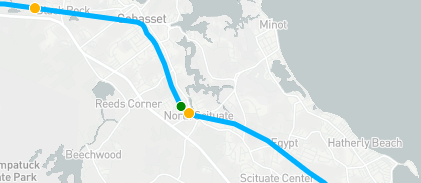
\includegraphics[width=0.4\textwidth]{prozess/animate_one_vehicle}
      \caption{Interpolation eines Vehicles entlang seiner Polyline}
      \label{fig:prozess/animate_one_vehicle}
    \end{center}
  \end{figure} 

  Das Ergebnis lässt sich in Abbildung \ref{fig:prozess/animate_one_vehicle} betrachten. Das Vehicle wird als grüner und die Stationen als orangene Kreise dargestellt.
  
% subsection animieren_eines_vehicles_durch_interpolation (end)